
\section{Methodology}
\label{sec:methods}


\def\ue{\ensuremath{\vec{\tilde{u}}\earth}}
\def\nrot{\ensuremath{\vec{n}_{\omega}}}
\def\nacc{\ensuremath{\vec{n}_{a}}}


This work describes a method for correcting velocity measurements from a moving velocity sensor, $\umeas$, using independent measurements of that sensor's motion, $\uhead$, to remove the motion from the velocity measurements, and thus estimate the `motion corrected velocity':
\begin{align}
  \label{eqn:u_mot_def}
  \ue(t) & = \umeas(t) + \uhead(t) \qquad .
\end{align}
Note here that the `+'-sign is correct because head motion, $\uhead$, induces a measured velocity in the opposite direction of the head motion itself ($\umeas = \ue - \uhead$). This approach has been used to successfully correct sonic anemometer measurements of atmospheric turbulence \cite[e.g., ][]{Edson++1998, Miller++2008}.  In the ocean, previous works have utilized inertial motion sensors to quantify the motion of multiscale profilers for the purpose of measuring the full spectrum of oceanic shear \cite[]{Winkel++1996}, and to quantify the motion of thermistor sensors \cite[]{Moum+Nash2009b}, but the \cite{Edson++1998} approach has not been documented for moored ADV measurements.

The Microstrain IMU available in the Nortek Vector ADV measures the linear acceleration, $\Accel$, rotational motion, $\AngRt$, and orientation matrix, $\omat$, of the ADV pressure case in the Earth reference frame at every time step of the ADV's sampling. So long as the ADV head is rigidly connected to the IMU (i.e. the ADV pressure case), the motion of the ADV head is calculated from these signals as the sum of rotational and translational motion:
\begin{align}
  \label{eqn:uhead}
\begin{split}
  \uhead & = \urot + \uacc + \ulow \\
      & = \omatinv \cdot \AngRt^*(t)\times\l + \int \rangle \Accel(t)\langle_{f_{a}} \,\mathrm{d}t + \ulow
\end{split}
\end{align}
Here, $*$ superscripts denote quantities in the ADV's local coordinate system, and $\l$ is the vector from the IMU to the ADV head. $\omatinv$---the inverse of the orientation matrix---rotates vectors from the IMU to the Earth reference frame. The notation $\rangle \cdot \langle _{f_a}$ indicates a high-pass filtering operation at frequency $f_a$. The high-pass filter reduces low-frequency noise in $\Accel$---sometimes referred to as bias drift---that is amplified by integration \cite[]{Barshan+Whyte1995, Bevly2004, Gulmammadov2009}. $\ulow$ is the low-frequency translational motion that is unresolved by $\uacc$, and it is discussed in more detail below. Note that, to avoid double counting, $\ulow$ should be estimated by applying the complementary low-pass filter to the independent measurement of low-frequency motion. We use fourth order, zero-phase (bidirectional), Hanning filters for all filtering operations.

\begin{figure}
  \centering
  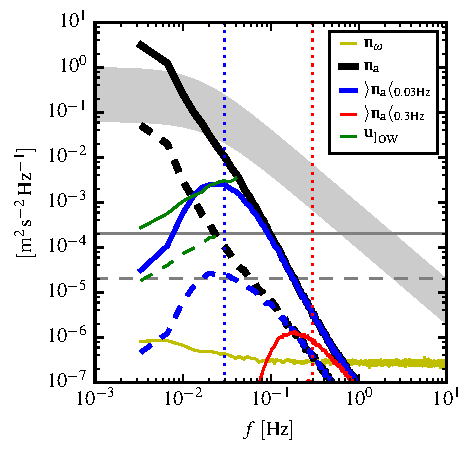
\includegraphics[width=\onewidth]{stationary_noise04}
  \caption{The spectral noise levels of rotational velocity ($\spec{\nrot}$, yellow) and translational velocity ($\spec{\nacc}$, black) estimated from an ADV-IMU resting motionless on a table. Solid and dashed lines indicate the horizontal and vertical components, respectively, of $\spec{\nacc}$ and $\spec{\ulow}$. The $\nacc$ signals are unfiltered (black), and high-pass filtered at 0.03 Hz (blue) and 0.3 Hz (red); vertical dotted lines indicate the filter frequency.  Green lines are an estimate of $\ulow$ for the TTM. Grey horizontal lines indicate the horizontal (solid) and vertical (dashed) Doppler noise levels of the ADV. The shaded region indicates the range of $\spec{u}$ presented in the next section.}
  \label{fig:stnoise}
\end{figure}

The noise levels of the IMU, $\nrot$ and $\nacc$, are computed from ADV-IMU data collected while the instrument was resting motionless on a table for several hours. Where, for this motionless dataset, the noise levels are defined according to \eqref{eqn:uhead} with $\nrot$ in place of $\urot$, and $\nacc$ in place of $\uacc$.  These are presented in Figure \ref{fig:stnoise} relative to the ADV spectra presented in following sections of this paper (grey shading), and relative to the Doppler noise levels of the ADV.

$\spec{\nrot}$ is equal in all three components, and so only one component is presented for simplicity (yellow). $\spec{\nrot}$ is several orders of magnitude lower than the velocity spectra we measured (grey region), and also more than an order of magnitude smaller than the Doppler noise levels of the ADV. Here we have used $\l=1$ m; which is the order-of-magnitude of the typical distance between the ADV head and the IMU. This indicates that the precision of $\urot$ (i.e. the angular rate sensor) is adequate for making corrections to ADV velocity measurements without filtering.

The noise level of $\spec{\uacc}$ (Figure \ref{fig:stnoise}, black), on the other hand, is dominated by a $f^{-2}$ slope that results from integrating the low-frequency noise in $\Accel$. The horizontal ($u$ and $v$) spectra of these noise levels are identical, and so we only present one of them for simplicity (solid lines). The vertical spectra noise levels are different because the signal-to-noise ratio is larger (dashed black lines). High-pass filtering reduces the low-frequency noise (blue and red) so that it does not contaminate motion correction, but any real motion that does exist at these frequencies is lost \cite[]{EgelandPhD2014, VanZwieten++2015}. This means there is a residual low-frequency translational motion, $\ulow$, that needs to be measured independently---or at the very least considered---when using ADV-IMU data from moving platforms. 

%\def\ulow{\ensuremath{\vec{u}_{\textnormal{low-SMB}}}}
For the SMB, the ADP bottom-track measured $\ulow$, and this measurement agrees with $\uacc$ over a narrow frequency band (see Part I, appendix A), indicating that the ADP and IMU are resolving the same motion. When this is the case, it is trivial to select a frequency in the middle of the spectral overlap (in this case, we choose $f_a=0.2$ Hz), and high-pass and low-pass filter $\uacc$ and $\ulow$, respectively, then sum to estimate total translational motion. This process gives a noteworthy improvement in the shape of $\spec{u}$ and $\spec{v}$ for the SMB when compared to assuming $\ulow=0$ (not shown). This indicates that ADP bottom-track measurements are important for resolving turbulence spectra from the SMB platform. 

%\def\ulow{\ensuremath{\vec{u}_{\textnormal{low-TTM}}}}
The position of the TTM ADV can be estimated, relative to its base, by assuming the mooring acts like a rigid pole and using the IMU orientation matrix to estimate the pole's `lean'. The position obtained from this model can then be differentiated to estimate $\ulow$ (this model does not apply at high frequencies). Spectra of $\ulow$ estimated using this approach for the June 2014 TTM deployment (Figure \ref{fig:stnoise}, blue) are plotted up to the point where they cross their respective $\spec{\uacc}$ noise level (black).  Together, these two lines provide an `aggregate noise level' of translational velocity estimates for the TTM: the rigid pole estimate of $\ulow$ indicates the amplitude of unresolved motion at low-$f$ (blue), and $\spec{\uacc}$ indicates the limits of the IMU at high-$f$ (black). Coincidentally, $\spec{\uacc}$ filtered at $f_a = 0.03$Hz is not a terrible approximation for this aggregate noise level. Furthermore, because this aggregate noise level is more than an order of magnitude lower than the velocity spectra of interest (shaded region), the results of motion correction are essentially identical whether we use the rigid pole model to estimate $\ulow$, or if we simply assume that $\ulow = 0$. 

%\def\ulow{\ensuremath{\ue_\mathrm{low}}}

\begin{figure}[t]
  \centering
  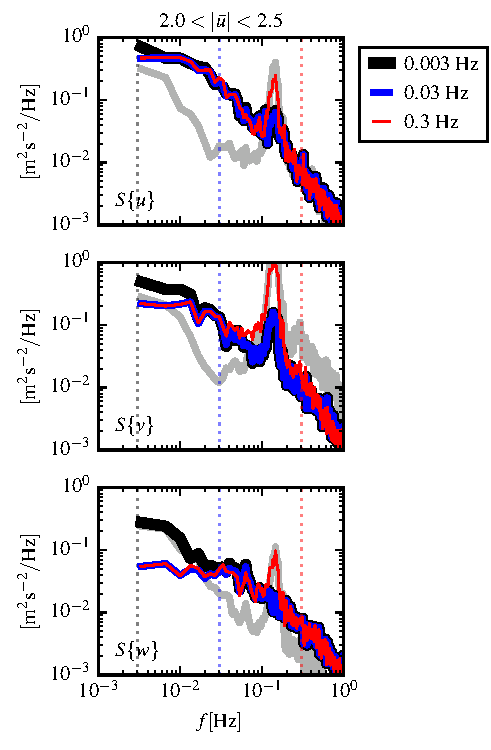
\includegraphics[width=\onewidth]{SpecFig04_filtering2}
  \caption{Motion-corrected velocity spectra, $\spec{\vec{u}}$, for a range of high-pass filter frequencies: $f_a= 0.3$ Hz (thin red), 0.03 Hz (blue), and 0.003 Hz (thick black). The vertical dashed lines indicate the filter frequency. The thick grey line is $\spec{\uhead}$ for $f_a=$ 0.003 Hz. The data are from the June 2014 TTM deployment when $2.0 < |\bar{u}| < 2.5\ \mathrm{ms^{-1}}$.
}
  \label{fig:filts}
\end{figure}

The choice of $f_a$ does influence the effectiveness of motion correction (Figure \ref{fig:filts}). When $f_a$ is too high (e.g., 0.3  Hz, red), the high-pass filter removes resolved motion from $\uhead$ that could be used to correct velocity measurements. In particular, notice that the amplitude of the 0.15 Hz peak---which is clearly the result of motion contamination (grey line)---is reduced significantly when we preserve more $\uhead$ information by reducing the high pass filter frequency to $f_a = 0.03$ Hz. Further reducing $f_a$ to $0.003$ Hz does not reduce the peak further, but does increase the amplitude of the spectra at low-frequency. This low-$f$ increase is the IMU-accelerometer's low-frequency bias drift (Figure \ref{fig:stnoise}) returning to contaminate the motion correction method.

Based on the above, we conclude that $f_a = 0.03$ Hz is a convenient `middle' frequency that reduces accelerometer bias-drift without destroying resolved motion of the TTM.  The same $f_a=0.03$ Hz filter was selected, based on a similar analysis, for the turbulence torpedo. The reader is likely to notice that the $0.15$ Hz peak is not completely removed by motion correction, especially for the $v$ component (Figure \ref{fig:filts}, middle panel). We will discuss this `persistent motion contamination' further in the following section.

Thus, we find that filter selection involves a trade-off between filtering out the bias drift noise at low-frequencies while not filtering out measured motion at high frequencies. In general, this will depend on the dynamics of the platform used to support the ADV, and the intensity of the turbulence being measured. When an independent measurement of $\ulow$ is available the cross-coherence with $\uacc$ can indicate a region of spectral overlap, and $f_a$ can be selected at the midpoint. Lacking a reliable estimate of $\ulow$,  the value of $f_a$ that produces the lowest $\tke$ estimates is likely the best. 

Additional details on motion correction---including a detailed accounting of the distinct coordinate systems of the IMU, ADV pressure case, and ADV head---can be found in \cite{Kilcher++2016}. Open-source Python tools for performing motion correction of ADV-IMU data---including scripts that write processed data in Matlab and tabulated formats---are available at \url{http://lkilcher.github.io/dolfyn/}.

\def\ue{\ensuremath{\vec{u}\earth}}

%%% Local Variables:
%%% mode: latex
%%% TeX-master: "Kilcher_etal_IMU-ADV"
%%% End:
